\section{Getting Started}

\subsection{Insertion Sort}

\begin{description}

  \descitem{2.1-1} {\itshape Using Figure 2.2 as a model, illustrate the operation of {\sc Insertion-Sort} on the array $A = \langle 31, 41, 59, 26, 41, 58 \rangle$.}

    \begin{ex}
      \begin{figure}[H]
        \centering
        \begin{subfigure}[t]{.45\textwidth}
          \centering
          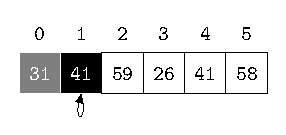
\includegraphics[scale=1]{img/2_1-1/2_1-1_1.pdf}
          \caption{}\label{fig:2_1-1_1}
        \end{subfigure}
        \begin{subfigure}[t]{.45\textwidth}
          \centering
          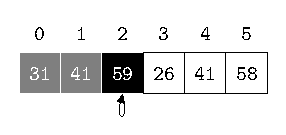
\includegraphics[scale=1]{img/2_1-1/2_1-1_2.pdf}
          \caption{}\label{fig:2_1-1_2}
        \end{subfigure}
        \begin{subfigure}[t]{.45\textwidth}
          \centering
          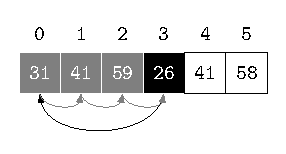
\includegraphics[scale=1]{img/2_1-1/2_1-1_3.pdf}
          \caption{}\label{fig:2_1-1_3}
        \end{subfigure}
        \begin{subfigure}[t]{.45\textwidth}
          \centering
          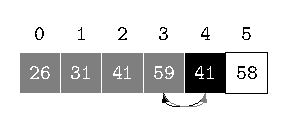
\includegraphics[scale=1]{img/2_1-1/2_1-1_4.pdf}
          \caption{}\label{fig:2_1-1_4}
        \end{subfigure}
        \begin{subfigure}[t]{.45\textwidth}
          \centering
          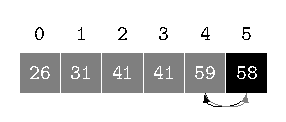
\includegraphics[scale=1]{img/2_1-1/2_1-1_5.pdf}
          \caption{}\label{fig:2_1-1_5}
        \end{subfigure}
        \begin{subfigure}[t]{.45\textwidth}
          \centering
          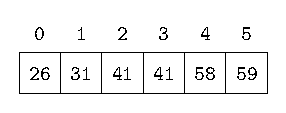
\includegraphics[scale=1]{img/2_1-1/2_1-1_6.pdf}
          \caption{}\label{fig:2_1-1_6}
        \end{subfigure}
        \caption{Tri par insertion sur le tableau $A = \langle 31, 41, 59, 26, 41, 58 \rangle$.} 
      \end{figure}
    \end{ex}

\descitem{2.1-2} {\itshape Rewrite the {\scshape Insertion-Sort} procedure to sort into non-increasing instead of non-decreasing order.}
    \begin{ex}
\begin{codebox}
\Procname{\algo{Decr-Insertion-Sort}$(A)$}
  \li \For $j \gets 2$ \To $\attrib{A}{length}$
  \li \Do
  $\id{key} \gets A[j]$
  \li \Comment Insert $A[j]$ into the sorted sequence
  $A[1 \twodots j-1]$.
  \li $i \gets j-1$
  \li \While $i > 0$ and $A[i] < \id{key}$
  \li \Do
  $A[i+1] \gets A[i]$
  \li $i \gets i-1$
  \End
  \li $A[i+1] \gets \id{key}$
  \End
\end{codebox}
\end{ex}


\descitem{2.1-3} {\itshape Consider the {\bfseries searching problem}:

  {\bfseries Input:} A sequence of $n$ numbers $A = \langle a_1, a_2, \ldots, a_n \rangle$ and a value $v$.

  {\bfseries Output:} An index $i$ such that $v = A[i]$ or the special value \const{nil} if $v$ does not appear in $A$.

Write pseudocode for {\bfseries linear search}, which scans through the sequence, looking for $v$. Using a loop, prove that your algorithm is correct. Make sure that your loop invariant fulfills the three necessary properties.}
  \begin{ex}
  \begin{codebox}
  \Procname{\algo{Linear-Search}$(A, v)$}
    \li $i\gets1$
    \li \While $i \le \attrib{A}{length}$ and $A[i]\ne v$
    \li \Do $i = i+1$ \End
    \li \If $i \le \attrib{A}{length}$ 
    \li \Then \Return $i$
    \li \Else
    \li \Return \const{nil}
    \End
    \end{codebox}
\begin{itemize}
  \item Initialisation : $i = 1$

    $[1 \twodots i-1]$ est vide, donc ne contient pas $v$.
  \item Conservation

    Pour tout $1\le i\le \attrib{A}{length}$, pour la boucle $i$, on a $[1 \twodots i-1]$ ne contenant pas $v$. Le corps de la boucle est execut\'e si et seulement si $A[i] \ne v$ et que $i \le \attrib{A}{length}$. Dans ce cas, avant l'it\'eration $i+1$, le sous-tableau $[1 \twodots i]$ ne contient pas $v$.
  \item Terminaison

    Il y a deux cas de terminaison :
    \begin{itemize}
      \item[$\bullet$]  quand $i = \attrib{A}{length}+ 1$, l'algorithme retourne \const{nil} et l'invariant de boucle confirme (en subtituant $i$ par $\attrib{A}{length}+1$) que le tableau $[1 \twodots \attrib{A}{length}]$ ne contient $v$;
      \item[$\bullet$] il existe un $1 \le i \le \attrib{A}{length}$ tel que $A[i] = v$, l'invariant de boucle dit que $[ 1 \twodots i-1]$ ne contient pas $v$, ce qui est vraie. Dans ce cas l'algorithme retourne $i$.
    \end{itemize}
\end{itemize}

\end{ex}

\descitem{2.1-4} {\itshape Consider the problem of adding two $n$-bit binary integers, stored in two $n$-element arrays $A$ and $B$. The sum of the two integers should be stored in binary form in an $(n+1)$-element array $C$.  State the problem formally and write pseudocode for adding the two integers.}

  \begin{ex}\\
    {\bfseries Input:} Deux nombres binaires $a$ et $b$ sous forme de vecteur $A = \langle a_1, \ldots, a_n \rangle$ et $B = \langle b_1, \ldots, b_n \rangle$ tel que pour tout $i \in \llbracket 1,n \rrbracket, a_i, b_i \in \{0,1\}$. Avec l'indice $i=1$ d\'esignant le bit le plus significant.

    {\bfseries Output:} Le vecteur $C = \langle c_1, \ldots, c_{n+1} \rangle$ qui repr\'esente $c = a+b$ en binaire.
    
    \begin{codebox}
    \Procname{ \algo{Add-Binary-Integer}$(A, B)$}
      \li $\id{carry} \gets 0 $
      \li \For $i=n$ \Downto $1$ \Do
      \li $\id{tmp} \gets A[i] + B[i] + \id{carry}$
      \li $C[i+1] \gets \id{tmp} \mod 2$
      \li $\id{carry} \gets \id{tmp}/2$\End
      \li $C[i] \gets \id{carry}$
    \end{codebox}
    
  \end{ex}
\subsection{Analyzing algorithms}

\descitem{2.2-1} {\itshape Express the function $n^3/1000-100n^2-100n+3$ in terms of $\Theta$-notation.}
  \begin{ex}
    $\Theta(n^3)$
  \end{ex}

\descitem{2.2-2} {\itshape
  Consider sorting $n$ numbers stored in array $A$ by first finding the smallest element of $A$ and exchanging it with the element in $A[1]$. Then find the second smallest element of $A$, and exchange it with $A[2]$. Continue in this manner for the first $n-1$ elements of $A$. Write pseudocode for this algorithm, which is known as {\bfseries selection sort}. What loop invariant does this algorithm maintain? Why does it need to run for only the first $n-1$ elements, rather than for all $n$ elements? Give the best-case and worst-case running times of selection sort in $\Theta$-notation.}

  \begin{ex}
    \begin{codebox}
    \Procname{\algo{Selection-Sort}$(A)$}
       \li \For $i = 1$ \To $n-1$ \Do
       \li \id{min \gets i}
       \li \For $j = i+1$ \To $n$ \Do
       \li \If $A[\id{min}] > A[j]$ \Then
       \li $\id{min} \gets j$ \End \End
       \li \If $\id{min} \ne j$ \Then
       \li \func{swap}(A, \id{min}, j) \End \End% TODO: add swap function
    \end{codebox}

    \begin{itemize}
      \item Invariant de boucle : 

        Le tableau $[1 \twodots i-1]$ est tri\'e avant la $i$\`eme it\'eration et tous les \'el\'ements dans $[i \twodots n]$ sont sup\'erieurs \`a ceux dans $[1\twodots i-1]$.

      \item \`A la $n-1$ it\'eration, le tableau $[1\twodots n-2]$ est tri\'e, il ne reste plus qu'\`a comparer $A[n-1]$ et $A[n]$.

     \item Temps d'ex\'ecution :
        \begin{itemize}
          \item[$\bullet$] Cas optimal : $A$ d\'ej\`a tri\'e, $\Theta(n^2)$ ;
          \item[$\bullet$] Cas le plus d\'efavorable : $A$ tri\'e de fa\c{c}on d\'ecroissante, $\Theta(n^2)$.
        \end{itemize}

    \end{itemize}

  \end{ex}

\descitem{2.2-3} {\itshape Consider linear search again (see Exercise 2.1-3). How many elements of the input sequence need to be checked on the average, assuming that the element being searched for is equally likely to be any element in the array? How about in the worst case ? What are the average-case and worst-case running times of linear search in $\Theta$-notation? Justify your answers.}

  \begin{ex}
    \begin{itemize}
      \item Cas moyen : $\frac{1}{n}\sum_{i=1}^ni = \frac{n+1}{2}$ ;
      \item Cas le plus d\'efavorable : $n+1$.
    \end{itemize}
    Donc $\Theta(n)$ dans les deux cas.
  \end{ex}

\descitem{2.2-4} {\itshape How can we modify almost any algorithm to have a good best-case running time?}

  \begin{ex}
    Tester au d\'ebut de l'algorithme la nature de l'entr\'ee, si celle-ci v\'erifie une certaine condition, retourner un r\'esultat calcul\'e pr\'ealablement. 
  \end{ex}

\end{description}

\subsection{Designing algorithms}

\begin{description}
  \descitem{2.3-1} {\itshape Using Figure 2.4 as a model, illustrate the operation of merge sort on the array $A =\\ \langle 3, 41, 52, 26, 38, 57, 9, 49\rangle$}.

    \begin{ex}
      \begin{figure}[H]
          \definecolor{merge}{RGB}{230, 211, 221}
        \centering
          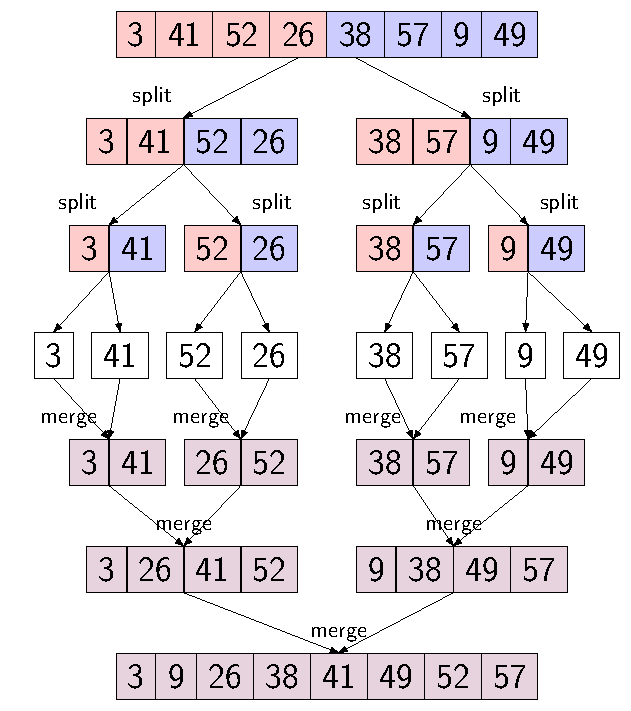
\includegraphics[scale=1]{img/2_3-1/2_3-1.pdf}
        \caption{Tri fusion sur le tableau $A =\langle 3, 41, 52, 26, 38, 57, 9, 49\rangle$.\\
          \raisebox{2.5pt}{\protect\tikz{\protect\draw[color=blue!20, line width=3pt] (0,0) -- (0.4,0);}} éléments de droite
          \raisebox{2.5pt}{\protect\tikz{\protect\draw[color=red!20, line width=3pt] (0,0) -- (0.4,0); }} éléments de gauche
          \raisebox{2.5pt}{\protect\tikz{\protect\draw[color=merge, line width=3pt] (0,0) -- (0.4,0);  }} éléments fusionnés (ordonné).}
      \end{figure}
      
    \end{ex}

  \descitem{2.3-2} {\itshape Rewrite the \textsc{Merge} procedure so that it does not use sentinels, instead stopping once either array $L$ or $R$ has had all its elements copied back to $A$ and then copying the remainder of the other array back into $A$.}

    \begin{ex}
      \begin{codebox}
      \Procname{\algo{Merge}$(A, p, q, r)$}
        \li $n_1 \gets q - p + 1$
        \li $n_2 \gets r - q$
        \li Let $L[1\twodots n_1]$ and $R[1\twodots n_2]$ be new arrays
        \li \For $i = 1$ \To $n_1$ \Do
        \li $L[i] \gets A[p + i -1]$ \End
        \li \For $j = 1$ \To $n_2$ \Do
        \li $R[j] \gets A[q + j]$ \End
        \li $i = 1$
        \li $j = 1$
        \li \For $k = p$ \To $r$ \Do
        \li \If $ j == n_2+1$ or  ($i \le n_1$ and $L[i] \le R[j]$) \Then
        \li $A[k] = L[i]$
        \li $i = i+1$
        \li \Else 
        \li $A[k] = R[j]$
        \li $j = j+1$\End \End
      \end{codebox}
    \end{ex}

  \descitem{2.3-3} {\itshape Use mathematical induction to show that when $n$ is an exact power of $2$, the solution of the recurrence 
    \[T(n) = \left\{
      \begin{array}{ll}
        2 & \text{ if } n = 2,\\
        2T(n/2)+n & \text{ if }n = 2^k, \text{ for } k> 1\\
      \end{array}
    \right.\]
  is $T(n) = n\lg n$.}

    \begin{ex}
      Soit $n = 2^p$, avec $p \in \N^*$.
      \begin{itemize}
        \item \ul{Initialisation} : $T(2) = 2\lg 2 = 2$ est vraie.
        \item \ul{H\'er\'edit\'e} : Soit $k < p$ et supposons que $T(2^k) = 2^k\lg 2^k = 2^kk$.

          Alors $T(2^{k+1}) = 2T(2^k)+2^{k+1} = 2^{k+1}(k+1)$.
        \item \ul{Conclusion} : Pour tout $p \in \N^*$, on a bien $T(2^p) = 2^p p$.
      \end{itemize}
    \end{ex}

  \descitem{2.3-4} {\itshape We can express insertion sort as a recursive procedure as follows. In order to sort ${ A = [1 \twodots n]}$, we recursively sort $A = [1 \twodots n-1]$ and then insert $A[n]$ into the sorted array ${A[1 \twodots n-1]}$ Write a recurrence for the running time of this recursive version of
insertion sort.}

\begin{ex}
  \[T(n) = \left\{
    \begin{array}{ll}
    \Theta(1) & \text {if } n = 1\\
      T(n-1) + \Theta(n) & \text{otherwise}\\ 
    \end{array}
  \right.\]
\end{ex}

\descitem{2.3-5} {\itshape Referring back to the searching problem (see Exercise 2.1-3), observe that if the sequence $A$ is sorted, we can check the midpoint of the sequence against and eliminate half of the sequence from further consideration. The {\bfseries binary search} algorithm repeats this procedure, halving the size of the remaining portion of the sequence each time. Write pseudocode, either iterative or recursive, for binary
  search. Argue that the worst-case running time of binary search is $\Theta (\lg n)$.}
  \begin{ex}
    \begin{codebox}
      \Procname{\algo{Rec-Bin-Search}$(A,p,q,v)$}
      \li $\id{mid} \gets \lfloor(p+q)/2\rfloor$
      \li \If $A[\id{mid}] < v$ \Then
      \li $\textsc{Rec-Bin-Search}(A, r+1, q, v)$ \End
      \li \Else \If $A[\id{mid}] > v$ \Then
      \li  $\textsc{Rec-Bin-Search}(A, p, \id{mid}-1, v)$ \End
      \li \Else \If $A[\id{mid}]  == v$ \Then
      \li \Return \id{mid}
      \li \Else 
      \li \Return \const{nil} \End
    \end{codebox}

    Calculons le temps d'ex\'ecution au cas le plus d\'efavorable. On a :
    \[T(n) = \left\{ 
      \begin{array}{ll}
        \Theta(1) & \text{if } n = 1\\
        T(n/2) + \Theta(1) & \text{otherwise}
      \end{array}
    \right..\]
    Supposons que $n = 2^p$, alors par la m\'ethode d'arbre r\'ecursive, on a un arbre d\'eg\'en\'er\'e de hauteur $p$ dans lequel chaque n\oe ud est \'etiquet\'e par une constante $c$. Il suffit donc de calculer 
    \begin{align*}
      \sum_{i=0}^{p}c &= (p+1)c\\
     &= (\lg n + 1)c\\
     &= \Theta(\lg n).
    \end{align*}
  \end{ex}

\descitem{2.3-6} {\itshape Observe that the {\bfseries while} loop of lines $5$–$7$ of the {\scshape Insertion-Sort} procedure in Section 2.1 uses a linear search to scan (backward) through the sorted subarray $A[1 \twodots j-1]$. Can we use a binary search (see Exercise 2.3-5) instead to improve the overall worst-case running time of insertion sort to $\Theta(n \lg n)$?}

  \begin{ex}
    Non. Dans la boucle \textbf{tant que}, on effectue deux t\^aches :
    \begin{enumerate}
      \item la recherche lin\'eaire de l'emplacement auquel on ins\`ere l'\'el\'ement : $\Theta (n)$ ;
      \item le d\'ecalage de tous les \'el\'ements apr\`es cet emplacement : $\Theta (n)$.
    \end{enumerate}
    Remplacer la recherche lin\'eaire par la recherche dichotomique am\'eliore la premi\`ere t\^ache en temps logarithmique. N\'eanmoins, le d\'ecalage toujours en $\Theta(n)$, cause un temps quadratique \`a l'algorithme.
  \end{ex}

\item[2.3-7 $\star$] {\itshape Describe a $\Theta (n \lg n)$-time algorithm that, given a set $S$ of $n$ integers and another integer $x$, determines whether or not there exist two elements in $S$ whose sum is exactly $x$.}

  \begin{exrev}
    
  \end{exrev}

\end{description}

\subsection{Problems}

\begin{description}
  \descitem{2-1} {\bfseries \itshape Insertion sort on small arrays in merge sort}

    {\itshape Although merge sort runs in $\Theta(n \lg n)$ worst-case time and insertion sort runs in $\Theta(n^2)$ worst-case time, the constant factors in insertion sort can make it faster in practice for small problem sizes on many machines. Thus, it makes sense to {\bfseries coarsen} the leaves of the recursion by using insertion sort within merge sort when subproblems become sufficiently small. Consider a modification to merge sort in which $n=k$ sublists of length $k$ are sorted using insertion sort and then merged using the standard merging mechanism, where $k$ is a value to be determined.
      \begin{Al}
        \item Show that insertion sort can sort the $n=k$ sublists, each of length $k$, in $\Theta (nk)$  worst-case time.
        \item Show how to merge the sublists in $\Theta (n\lg (n/k))$ worst-case time.
        \item Given that the modified algorithm runs in $\Theta(nk + n\lg (n/k))$ worst-case time, what is the largest value of $k$ as a function of $n$ for which the modified algorithm has the same running time as standard merge sort, in terms of $\Theta$-notation?
        \item How should we choose k in practice?
      \end{Al}
    }

    \begin{pbrev}
      
    \end{pbrev}

  \descitem{2-2} {\bfseries \itshape Correctness of bubblesort}

    {\itshape Bubblesort is a popular, but inefficient, sorting algorithm. It works by repeatedly
    swapping adjacent elements that are out of order.}

    \begin{pbrev}
      
    \end{pbrev}

  \descitem{2-3} {\bfseries \itshape Correctness of Horner’s rule}

    {\itshape The following code fragment implements Horner’s rule for evaluating a polynomial}

    \begin{pbrev}
      
    \end{pbrev}

  \descitem{2-4} {\bfseries \itshape Inversions}

    \begin{pbrev}
      
    \end{pbrev}

\end{description}

